\subsection{Heurística constructiva de cluster-first, route-second, clusterizando con algoritmo de Sweeping} \label{subsection:sweep}
\subsubsection{El algoritmo}
La solución al Problema de Enrutamiento de Vehículos con Capacidad mediante este algoritmo se divide en dos partes fundamentales: \textbf{1.} la clusterización y \textbf{2.} la búsqueda de un camino mínimo. La clusterización de los vértices de un grafo puede ser llevada a cabo de distintas maneras. En trabajos anteriores hemos utilizado el algoritmo de Kruskal y el algoritmo de Prim para obtener árboles generadores mínimos sobre los cuales se ejercían exploraciones vecinales y consecuentes podas hasta obtener una clusterización válida. Otros enfoques, por ejemplo, utilizan técnicas como la clusterización por $k-medians$ para agrupar nodos cercanos. Las alternativas son enormes. En este documento utilizamos el \textit{Sweep Clustering Algorithm} para producir los conjuntos de vértices euclidianamente cercanos.

\vskip 8pt

El concepto de \textit{sweeping} es fácil. Será conveniente distribuir los nodos en representación polar $(r, \theta)$ donde $r$ es la distancia del vértice al origen de coordenadas y $\theta$ el ángulo polar. De esta manera, – desde el nodo depósito – comenzamos proyectando un haz de luz y con él realizaremos un barrido en sentido anti-horario. Guardaremos en un conjunto todos los vértices que el haz vaya tocando hasta que la suma de todas sus demandas supere la capacidad de un camión. Cuando esto suceda, terminaremos de agregar elementos a este conjunto y crearemos otro donde seguiremos introduciendo nodos que se crucen con nuestro haz hasta volver a superar la capacidad máxima de un camión. Este procedimiento se sigue repitiendo hasta que no queden más nodos por asignar a un conjunto. Estos conjuntos \textbf{representan los clusters} y lo que estamos agrupando son \textbf{nodos angularmente cercanos entre sí} que \textbf{puedan ser satisfechos por un sólo camión}. Es decir, en nuestro esquema, satisfacer cada cluster será responsabilidad de uno y sólo un camión. Esta heurística pretende agrupar todos los clientes cercanos minimizando la distancia recorrida por los camiones. Es necesario notar que la forma final de los clusters tienden a tener un parecido natural a los pétalos de una flor. En general, las rutas con forma de pétalos son una característica geométrica muy común en las soluciones del Problema de Enrutamiento de Vehículos \textit{(Ryan et al. 1993a)}.

\vskip 8pt

Por último, ya sabemos qué vértices serán visitados por qué camiones, sin embargo, no sabemos en qué orden. Este problema es una instancia del \textbf{Problema del Viajante} y se decidió atacarla con \textbf{Nearest Neighbours Algorithm}, una heurística constructiva cuya solución fabrica de manera golosa que, como el nombre lo indica, consiste en visitar el vecino más cercano. A continuación procederemos a describir los pasos del algoritmo general:

\begin{description}
\item[Paso 1.] Polarización de las coordenadas cartesianas
\item[Paso 2.] Ordenamiento creciente de las coordenadas por sus ángulos polares
\item[Paso 3.] Averiguación del ángulo de \textit{menor densidad}
\item[Paso 4.] Ordenamiento creciente de las coordenadas por sus ángulos polares desde el \textit{ángulo de menor densidad}
\item[Paso 5.] Construcción de los \textit{clusters} mediante un \textit{sweeping} en sentido anti-horario
\item[Paso 6.] Aplicación de la heurística \textit{Nearest Neighbours} sobre cada cluster para la generación de rutas
\end{description}

Hay un detalle extra en la lógica de nuestro algoritmo llamado el \textbf{ángulo de menor densidad}. Para explicar esta medida, primer debemos explicar sus causas: en nuestro esquema inicial, planteamos un barrido de nodos para el armado de los \textit{clusters}. Lo que hemos omitido hasta ahora es que este barrido debe comenzar en algún lugar, o específicamente, un ángulo. Si no seleccionásemos cuidadosamente este ángulo y decidiésemos iniciar el barrido en un ángulo $\theta$, podría suceder que la solución óptima (que intentamos aproximar heurísticamente) contenga un cluster que es partido a la mitad por el haz proyectado desde el depósito en el ángulo $\theta$, y debido al movimiento natural del sweeping – es decir, antihorario – sólo se registre una mitad del cluster y no la otra que \textbf{hubiera quedado del lado horario} de $\theta$. Esto concluiría en la concepción de otro cluster distinto al óptimo y, en consecuencia, la posterior alteración del resto de la clusterización de los nodos. Por esta razón introducimos la noción de \textbf{sweeping adaptativo} que consiste en comenzar el barrido desde el ángulo \textbf{menos favorable} para la ocurriencia de estas falencias en nuestro algoritmo, pues minimiza la posibilidad de interrumpir (o atravezar) un cluster óptimo con nuestro haz al proyectarlo en un ángulo donde se deduce heurísticamente una baja densidad poblacional de nodos. Este ángulo es el ángulo de menor densidad y se entiende como el ángulo que atraviesa a la mitad \textbf{el espacio más grande entre dos vértices consecutivos} del grafo. En otras palabras, para calcular este ángulo encontramos la distancia más grande entre dos nodos angularmente consecutivos y comenzamos nuestro sweeping ahí. Si $\theta_{1}$ y $\theta_{2}$ son dos vértices consecutivos con la mayor separación angular del grafo donde $\theta_{1}$ es encontrado primero por el barrido, definimos como $\alpha$ el ángulo de menor densidad que equivale a:

\begin{center}
\begin{displaymath}
\alpha = \left\{
\begin{array}{l l}
			\alpha_{1} + \frac{|\alpha_{1} - \alpha_{2}|}{2} & \text{si }\alpha_{1} < \alpha_{2}\\
			\alpha_{1} + \frac{|2*\pi - \alpha_{1} + \alpha_{2}|}{2} & \text{sino}\\
\end{array}
\right.
\end{displaymath}
\end{center}

Por otro lado, podemos acotar la complejidad espacial del algoritmo por $\bigO(n)$ porque siempre se trabaja con el conjunto de $n$ vértices y no más.

\subsubsection{Pseudo-código}
A continuación presentamos nuestras implementaciones con sus respectivas complejidades:

\begin{algorithm}[H]
\caption{\Comment $\mathcal{O}(????)$}
\begin{algorithmic}[1]
\Function{resolverCVRP}{Punto $deposito$, Conjunto de puntos $puntos$, Entero $capacidad$}
	\State \textbf{Buckets} $buckets \gets $\textbf{BucketSortPorDemanda}$(puntos)$ \Comment $\mathcal{O}(n + D)$
	\State \textbf{OrdenarCadaBucketPorCercaníaA}$(puntos, deposito)$ \Comment $\mathcal{O}(n*log(n))$
	\Statex
	\State \textbf{Entero} $vertices\_cubiertos \gets 0$
	\State \textbf{Lista de Camiones} $camiones \gets \varnothing$
	\State Insertar en $camiones$ un camión con capacidad $capacidad$ que empieza en $deposito$
	\Statex
	\While{$vertices\_cubiertos < |puntos|$}
		\State \textbf{Bucket} $bucket\_mas\_apto \gets$ \par
        \Statex[3] \textbf{EncontrarBucketMasApto}$(buckets, camiones, deposito, capacidad)$
		\State \textbf{Punto} $siguiente \gets$ \textbf{ExtraerVerticeMasApto}$(bucket\_mas\_apto, camiones)$
		\State Tomar el último camión agregado a $camiones$ y visitar el vértice $siguiente$
		\Statex
		\State $vertices\_cubiertos \gets vertices\_cubiertos + 1$
	\EndWhile

	\State \Return $camiones$
\EndFunction
\end{algorithmic}
\end{algorithm}

\vspace{10 pt}
\fbox{\parbox{0.9\textwidth}{
	Es necesario aclarar que el tipo de datos \textbf{Camión} lleva la cuenta de su stock disponible en forma de \textbf{Entero positivo} y los vértices que visita en un conjunto ordenado de \textbf{Lista de Puntos}. Además, llamamos un \textbf{Bucket} a una \textbf{Lista de Puntos} que comparten la misma demanda. Análogamente, llamamos \textbf{Buckets} a una \textbf{Lista de Buckets}, es decir, Buckets es un alias para una lista de lista de puntos. Hacemos este renombre para resaltar la diferencia entre una lista de puntos con la misma demanda (un bucket) y una lista de puntos cualquiera. El tipo de datos \textbf{Buckets} es obtenido a partir de la invocación de un \textbf{Bucket Sort} sobre una lista de puntos utilizando la demanda de cada vértice como valor comparativo.

	\vskip 8pt

	Como último, el valor $D$ mencionado en la complejidad temporal del \textbf{BucketSort} es la máxima demanda de un punto en la lista $puntos$.
}}
\vspace{10 pt}

\vskip 8pt
Esta función representa la globalidad de la heurística. Como fue mencionado en la introducción, el algoritmo comienza polarizando los puntos que inicialmente están representados en coordenadas cartesianas. Esto se realiza en $\bigO(n)$ pues se deben iterar todos los nodos en el grafo y, a partir de sus coordenadas $x$ e $y$, calcular sus valores polares y radiales. Luego, como cada vértice ya está polarizado, podemos ordenar cada uno por su cercanía al ángulo $0$ en radianes.

\begin{algorithm}[H]
\caption{\Comment $\mathcal{O}(n)$}
\begin{algorithmic}[1]
\Function{CalcularÁnguloDeSweeping}{Lista de puntos $puntos$}
	\State \textbf{Punto} $previo \gets puntos[0]$
	\State \textbf{Punto flotante} $\alpha$
	\State
	\For{Entero $i \gets 1 \dots |puntos|$}
	\Comment $\mathcal{O}(n)$

		\State \textbf{Entero} $index \gets i \ \% \ |puntos|$
		\State \textbf{Punto} $actual \gets puntos[index]$
		\Statex
		\If{distancia angular entre $previo$ y $actual$ es la más alta hasta ahora}
			\State $\alpha \gets $ ángulo medio entre $previo$ y $actual$
			\Comment $\mathcal{O}(1)$
		\EndIf
	\EndFor
	\Statex
	\State \Return $\alpha$
\EndFunction
\end{algorithmic}
\end{algorithm}
Ahora que sabemos qué vértice viene después de cuál en el barrido, averiguamos en qué ángulo debemos iniciar el \textit{sweep}. Esto lo hacemos en $\Theta(n)$ porque comparamos todos los vértices con su siguiente. Es importante notar el manejo del caso borde cuando se compara el vértice último vértice de la lista con el primero, pues si bien euclidianamente pueden estar casi al lado, al examinar sus ángulos podemos ver una diferencia enorme (pues el que esté por encima del eje $x$ tendrá un ángulo cercano a $0$, pero el que esté por debajo, a $2$). Esta situación se da cuando el primer vértice en el recorrido del \textit{sweep} tiene un ángulo mayor al segundo vértice detectado. Luego del cálculo, estamos en condiciones de generar los clusters porque ya disponemos del ángulo de inicio del barrido.

\begin{algorithm}[H]
\caption{\Comment $\mathcal{O}(n)$}
\begin{algorithmic}[1]
\Function{ConstruirClusters}{Lista de puntos $puntos$, Entero $capacidad$}
	\State \textbf{Lista de Cluster} $clusters \gets \varnothing$
	\State $clusters \gets \{\text{Nuevo \textbf{cluster} vacío}\}$
	\State \textbf{Entero} $stock\_actual \gets capacidad$
	\Statex
	\For{Punto $p$ en $puntos$}
	\Comment $\mathcal{O}(n)$
	
		\If{$stock\_actual < p.demanda$}
			\State $stock\_actual \gets capacidad$
			\State $clusters \gets \{\text{Nuevo \textbf{cluster} vacío}\}$
		\EndIf
		\Statex
		\State $stock\_actual \gets stock\_actual - p.demanda$
		\State Insertar $p$ en el último cluster agregado a $clusters$
	\EndFor
	\Statex
	\State \Return $clusters$
\EndFunction
\end{algorithmic}
\end{algorithm}
Aquí es donde se realiza el barrido cuyo costo asintótico temporal es exactamente $\Theta(n)$ porque – devuelta – se recorren todos los nodos. Aquí es donde sucede la distribución de vértices a clusters tal que todos los vértices en un cluster son: \textbf{(a)} angularmente consecutivos y \textbf{(b)} satisfacibles por un sólo camión, como ya fue explicado en la introducción al algoritmo.

\begin{algorithm}[H]
\caption{\Comment $\mathcal{O}(n^2*log(n))$}
\begin{algorithmic}[1]
\Function{ConstruirRutasAPartirDeClusters}{Lista de Clusters $clusters$, Punto $dep\acute{o}sito$, Entero $capacidad$}
	\State \textbf{Lista de camiones} $camiones$
	\State Agregar a $camiones$ un camión que comienza en $dep\acute{o}sito$ con capacidad $capacidad$
	\Statex
	\For{$cluster$ en $clusters$}
		\While{$clusters$ no sea vacío}
			\State \textbf{Camión} $\acute{u}ltimo\_cami\acute{o}n \gets$ último camión agregado en $camiones$
			\State \textbf{Punto} $\acute{u}ltimo\_punto \gets$ último nodo visitado por $acute{u}ltimo\_cami\acute{o}n$
			\Statex
			\State \textbf{Punto} $siguiente\_punto \gets$ 
			\Statex[5] \textbf{ExtraerVérticeMásCercanoA}$(cluster, \acute{u}ltimo\_punto)$
			\Comment $\mathcal{O}(n*log(n))$

			\State \textbf{Visitar} $siguiente\_punto$ con $\acute{u}ltimo\_cami\acute{o}n$
		\EndWhile
		\Statex
		\State \textbf{Visitar} $dep\acute{o}sito$ con $\acute{u}ltimo\_cami\acute{o}n$
		\State Agregar a $camiones$ un camión que empieza en $dep\acute{o}sito$ con capacidad $capacidad$
	\EndFor
	\Statex
	\State \Return $camiones$
\EndFunction
\end{algorithmic}
\end{algorithm}
El bucle \textit{for} se ejecuta $\bigO(|clusters|)$ veces, mientras que el \textit{while} se ejecuta $\bigO(|clusters| * |cluster|)$ veces. En síntesis, esta complejidad equivale a $\bigO(n)$ pues la suma de todas las dimensiones de todos los $cluster \in clusters$ da $n$. Pero hay un detalle: la función \textbf{ExtraerVérticeMásCercanoA} posee una complejidad cuasilineal en función de la entrada. Si bien la complejidad de esta invocación sería $\bigO(|cluster| * log(|cluster|))$, relajaremos la cota por $\bigO(n*log(n))$ por una cuestión de comodidad. Por lo tanto, la complejidad final de este subalgoritmo queda definida por $\bigO(n^2*log(n))$.

\begin{algorithm}[H]
\caption{\Comment $\mathcal{O}(n*log(n))$}
\begin{algorithmic}[1]
\Function{ExtraerVérticeMásCercanoA}{Cluster $cluster$, Punto $punto$}
	\State \textbf{Ordenar} decrecientemente los nodos de $cluster$ por cercanía angular a $punto$
	\Comment $\mathcal{O}(n*log(n))$

	\State \textbf{Punto} $m\acute{a}s\_cercano \gets$ último elemento de $cluster$
	\Comment $\mathcal{O}(1)$

	\State $cluster \gets cluster - \{m\acute{a}s\_cercano\}$
	\Comment $\mathcal{O}(1)$
	\Statex
	\State \Return $m\acute{a}s\_cercano$
\EndFunction
\end{algorithmic}
\end{algorithm}
Finalmente, la función \textbf{ExtraerVérticeMásCercanoA} toma un cluster y un punto, ordena decrecientemente el cluster por distancia euclideana a $punto$, toma el último elemento de la lista (es decir, el más cercano a $punto$) y lo retorna sin no antes eliminarlo de la lista en $\bigO(1)$ porque es el último elemento de la lista. La complejidad de esta función queda definida por el ordenamiento $\bigO(n*log(n))$ de la lista en la línea $2$.

\subsubsection{Análisis de desempeño}
En esta sección analizaremos las destrezas y debilidades del algoritmo en discusión, que posee al menos dos falencias importantes que pueden producir soluciones de deslucida calidad. A continuación las repasamos:

\subsubsubsection{El algoritmo de \textit{sweeping} no prevee el agotamiento de stock}
A medida que un cluster se va construyendo, la capacidad del camión que atenderá los clientes de este conjunto se va agotando, es decir, la sumatoria de las demandas de todos los clientes en el cluster se va aproximando al valor de la capacidad máxima de los camiones. En estos casos, sería ideal emprender la vuelta hacia el depósito con stock suficiente para satisfacer vértices en el camino. Una manera de entender este concepto es visualizar cada ruta como un pétalo, donde la punta del antófilo indica el comienzo del emprendimiento al depósito. De esta manera, se minimiza la distancia recorrida al volver al punto de inicio pero \textbf{satisfaciendo vértices en el proceso}. Desgraciadamente, el algoritmo es inconsciente de esta situación y, en el peor de los casos, puede agotar su stock muy lejos del depósito solamente por seguir a rajatabla la heurística de viajar al nodo angularmente más cercano, pagando una distancia muy alta para volver.

\vskip 8pt

Esta falencia puede ser mitigada con metaheurísticas como \textbf{Tabú Search} o \textbf{Annealing} a la hora de seleccionar el siguiente vértice a visitar, teniendo en cuenta el vecindario inmediato y la cantidad de stock sobrante en el camión.

\begin{figure}[H]
	\centering
	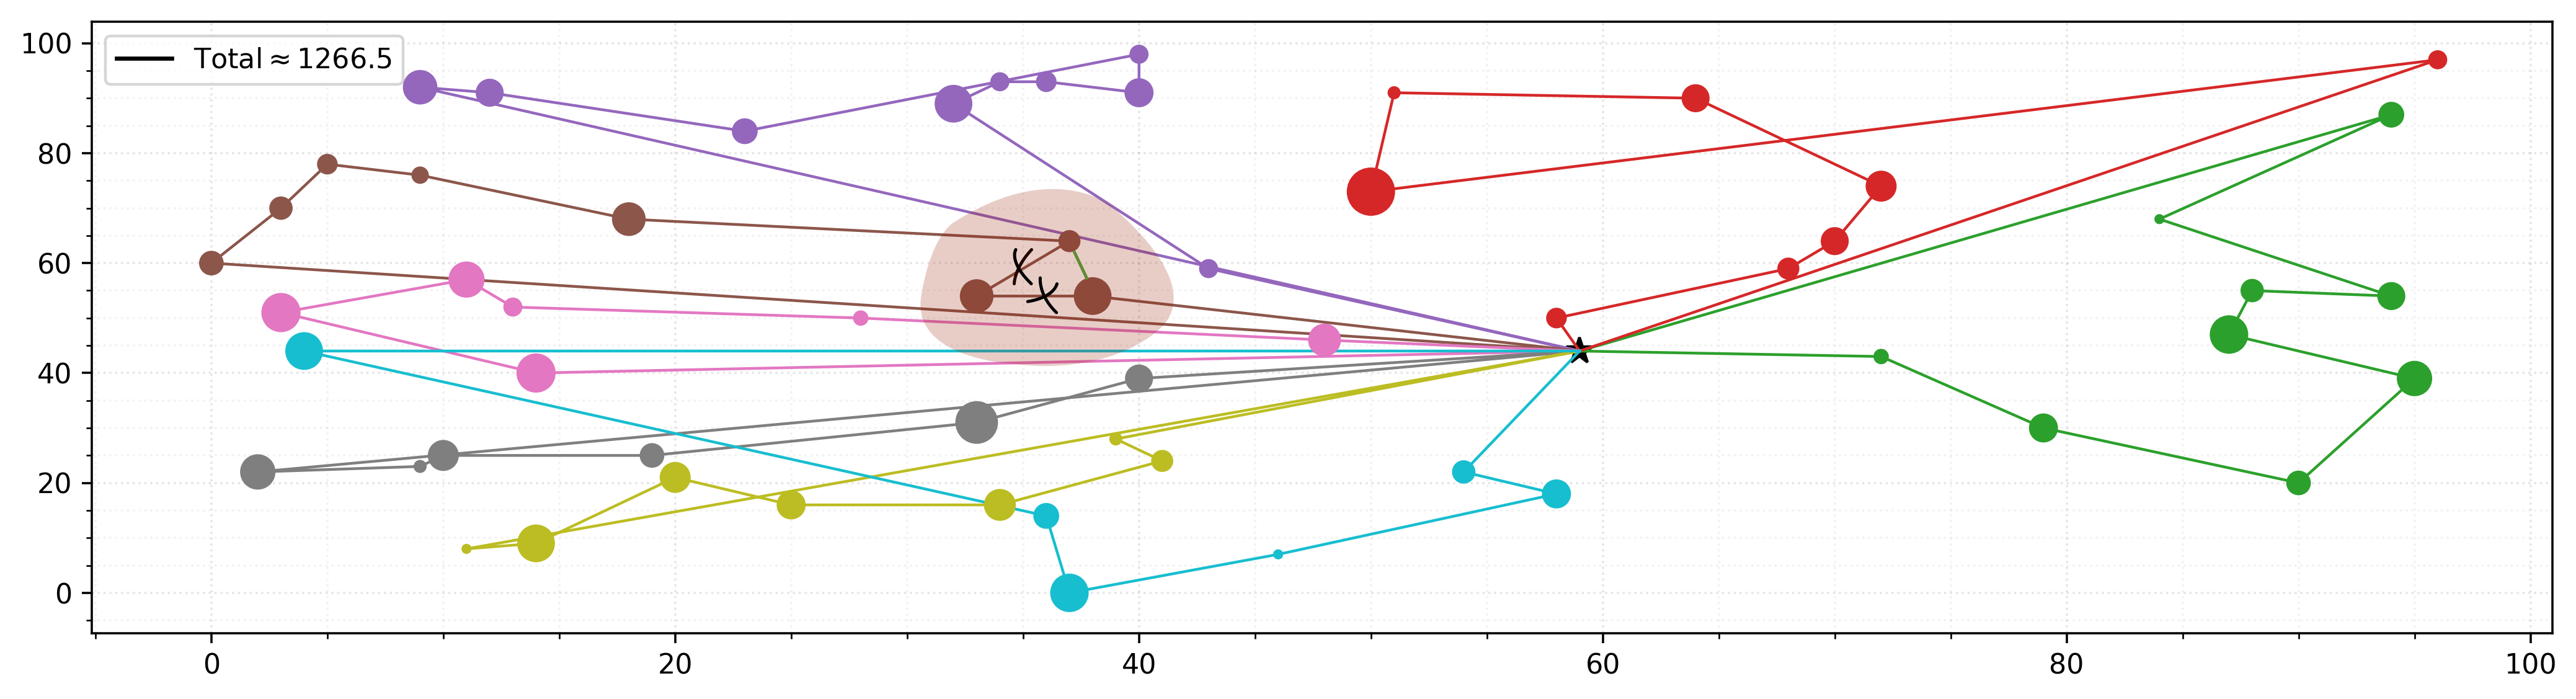
\includegraphics[width=1\textwidth]{sweep/A-n69-k9-emprender-vuelta}
	\caption{\footnotesize Error de optimización en la generación del camino (dataset A-n69-k9)}
	\label{fig:sweep-emprender-vuelta}
\end{figure}

En la figura \ref{fig:sweep-emprender-vuelta} se puede observar que en el camino marrón es posible obtener un mejor recorrido al eliminar los ejes marcados con una cruz y, en cambio, agregando la arista verde como figura en el gráfico. De esta manera quedaría un vértice $v$ sin conectar. Luego, si observamos el eje $e$ formado por el depósito y el nodo más alejado a él en esta ruta, podemos generar una subdivisión de la arista $e$ con el vértice $v$ concluyendo en un camino más óptimo. En resumen: la solución del gráfico \ref{fig:sweep-emprender-vuelta} posee una ruta que realiza un \textit{paso hacia atrás}, alejándose de los nodos que tiene que visitar después y tomando posesión de un cliente que podría haber sido visitado a la hora de \textbf{emprender la vuelta} hacia el depósito. Este ejemplo es uno de los muchos que puede suceder en esta familia de problemas.

\subsubsubsection{La heurística de \textit{TSP} puede ser muy golosa con las distancias}
Debido a que el orden de los clientes en los clusters es resuelto a través de la heurística \textit{Nearest Neighbours} que consiste en visitar el nodo inmediatamente más cercano sobre el cual se está parado, se puede perder el panorama general y cometer decisiones costosas para la calidad de la solución final. El ejemplo más recurrente se ve en la presencia de rutas con bucles o \textit{firuletes}, pues se produce una ``ida y vuelta'' innecesaria con total de visitar el nodo más cercano posible. Esto podría ser evitado utilizado alguna metaheurística como Annealing o Tabú Search para decidir a qué vértice saltar o utilizar una técnica como Lambda Exchange para optimizar e intentar eliminar estas manifestaciones del problema descripto. Analizaremos este fenómeno gráficamente:

% \newpage
\parindent0em
\begin{multicols}{2}[\columnsep2em]
		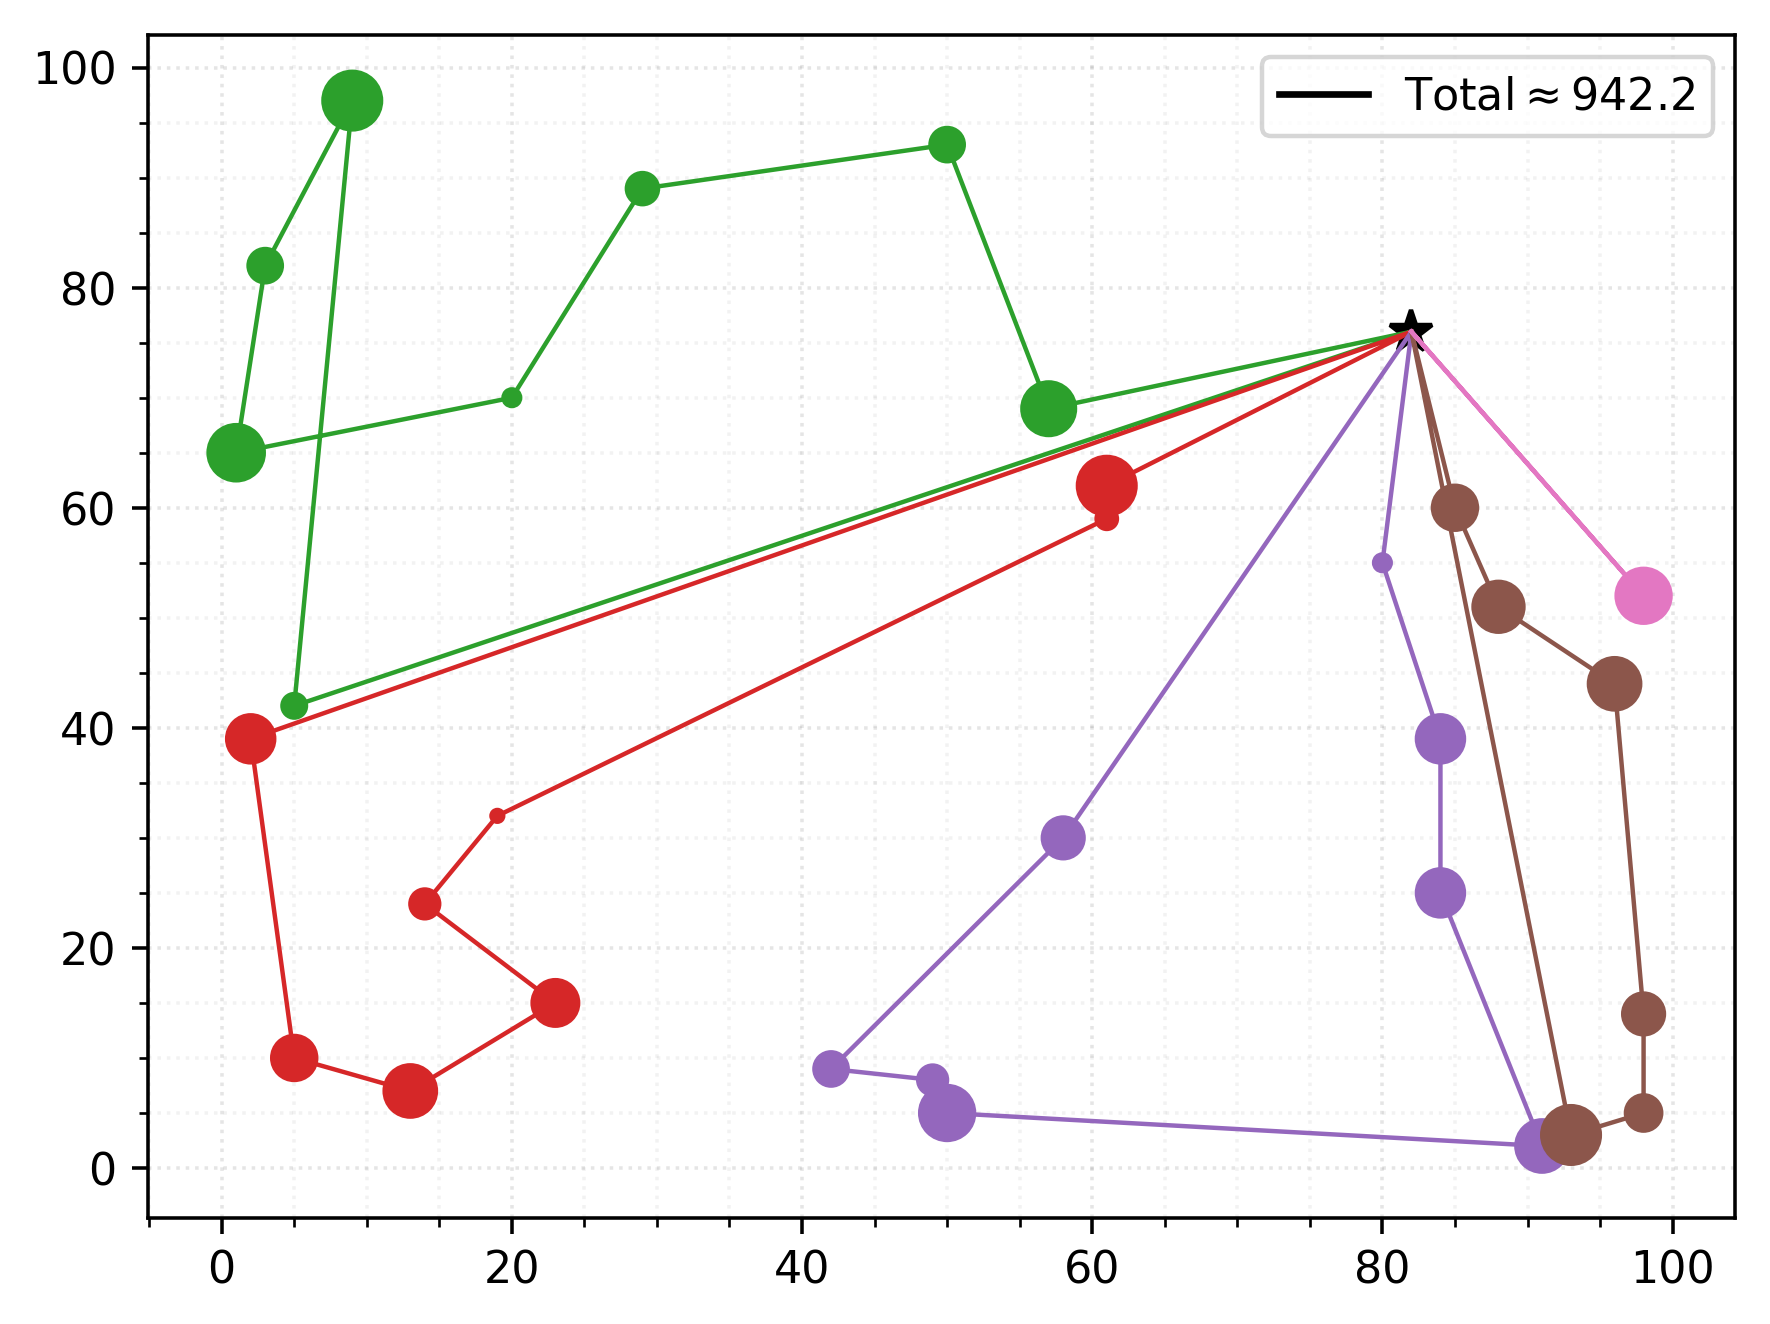
\includegraphics[width=0.48\textwidth]{sweep/sweep-A-n32-k5}
\columnbreak
	\begin{figure}[H]
		\caption{Circuito no óptimo en camino verde} \label{fig:sweep-A-n32-k5}
		\vskip 4pt
		En este ejemplo se puede ver claramente la aparición de un circuito en la ruta verde. Como ya fue explicado, este se debe a que el algoritmo de resolución del TSP busca los nodos inmediatamente más cercanos sin considerar otras alternativas (a priori más ineficientes) pero que a la larga resultan más óptimas. Al seguir a rajatabla la heurística de \textit{Nearest Neighbours}, se comete un error de \textit{tunnel view} y se ignoran alternativas más eficientes a la larga.
	\end{figure}
\end{multicols}

\subsubsubsection{Clusterización con sweeping adaptativo vs sin sweeping adaptativo}
En la figura \ref{fig:sweep-with-adaptative} se puede observar una clusterización correcta de los vértices. Los nodos recorridos por el camión verde son cercanos entre sí y lo mismo sucede con los del camión rojo. En cambio, en la figura \ref{fig:sweep-without-adaptative}, se puede observar cómo los clusters se interponen entre sí debido a que se comenzó a barrer angularmente sobre ángulo $0$, interrumpiendo a la mitad la concepción de un cluster óptimo.
\begin{figure}[H]
	\centering
	\begin{minipage}{0.48\textwidth}
		\centering
		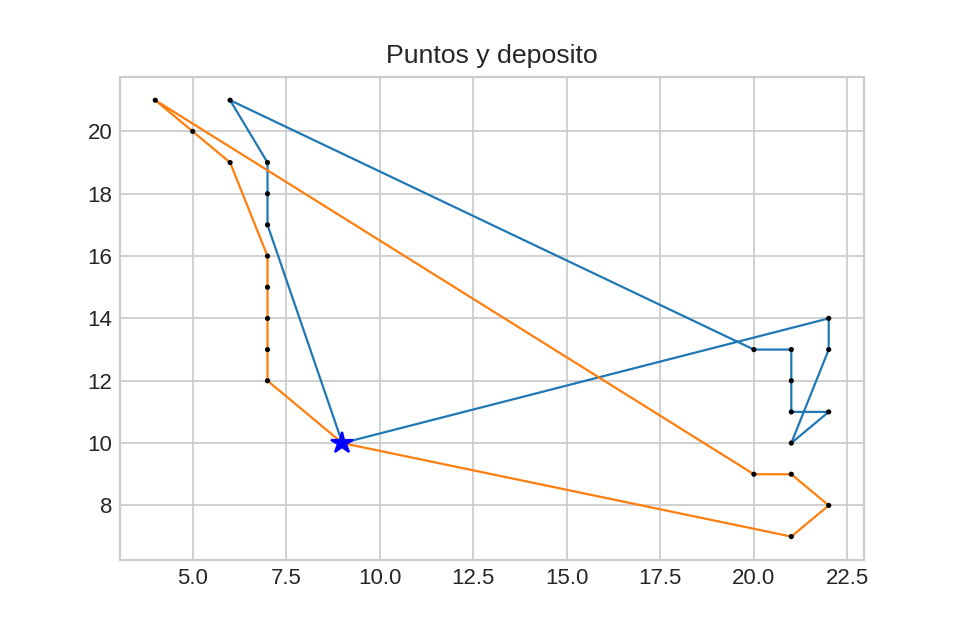
\includegraphics[width=1\textwidth]{sweep/sweep-without-adaptative}
		\caption{\footnotesize Sweeping no adaptativo}
		\label{fig:sweep-without-adaptative}
	\end{minipage}%
	\hspace{0.03\textwidth}
	\begin{minipage}{0.48\textwidth}
		\centering
		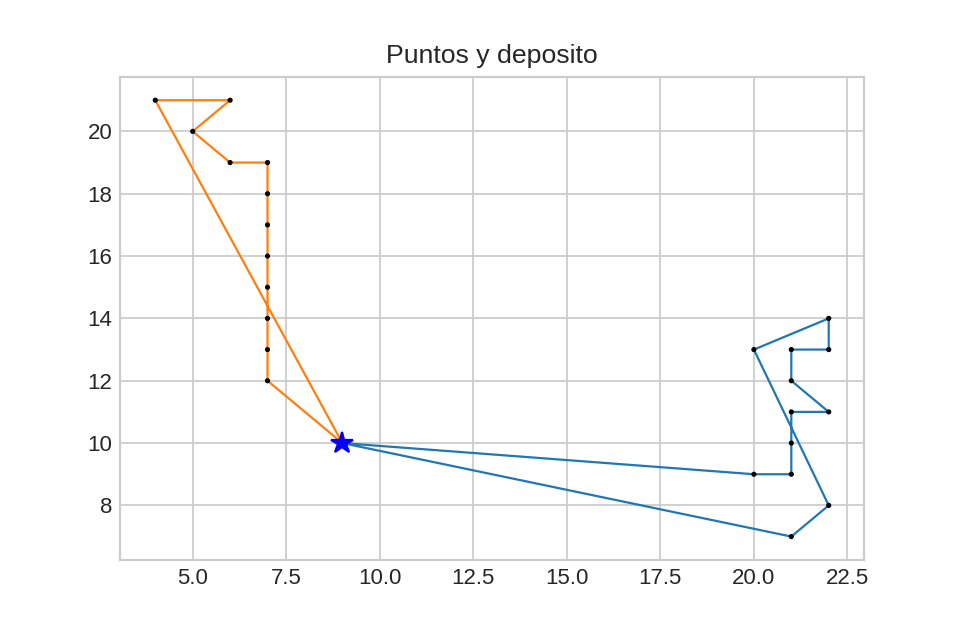
\includegraphics[width=1\textwidth]{sweep/sweep-with-adaptative}
		\caption{\footnotesize Sweeping adaptativo}
		\label{fig:sweep-with-adaptative}
	\end{minipage}%
\end{figure}

\subsubsubsection{El barrido angular puede clusterizar vértices muy lejanos entre sí}
Dada la clusterizaciónn de vértices $V=\{v_{1}, \dots, v_{n}\}$ realizada por la heurística de Sweeping donde, si bien está asegurado que la distancia angular desde el depósito entre todo $v_{i}$ y $v_{i+1}$ con $1 \leq i < n$ es mínima en todo el grafo, no está asegurado que la distancia euclidiana entre $v_{i}$ y $v_{i+1}$ sea mínima también. De hecho, la distancia entre $v_{i}$ y $v_{i+1}$ puede ser arbitraria. Sin embargo, al clusterizar ambos vértices juntos, estamos firmando un contrato donde un solo camión deberá proveer a ambos y esto puede ser extremadamente costoso por más que los recorridos sean realizados a fin de cuentas con una heurística de TSP. Veamos un ejemplo:

\begin{figure}[H]
	\centering
	\begin{minipage}{0.48\textwidth}
		\centering
		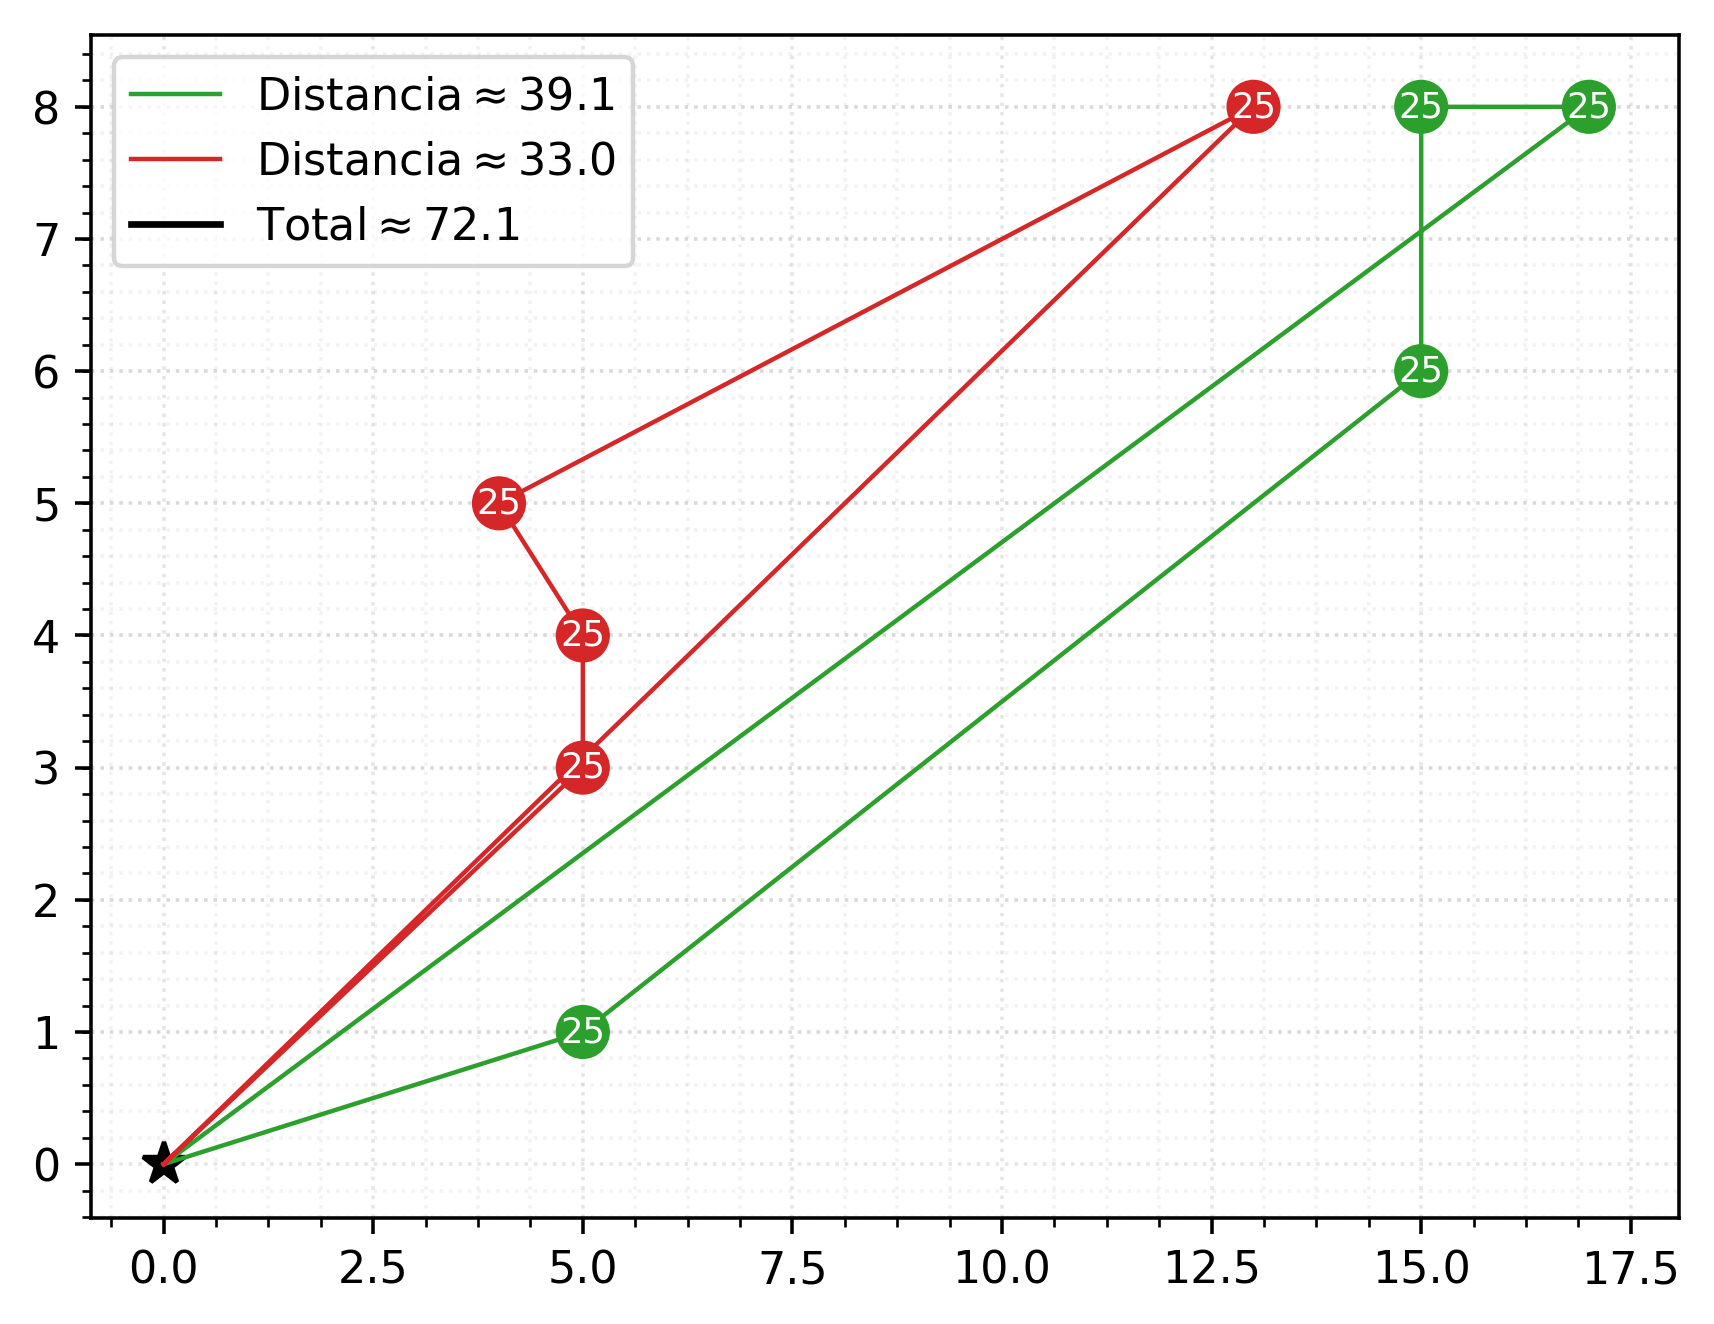
\includegraphics[width=1\textwidth]{sweep/sw-custom-n9-sweep-close-angular-far-euclidean}
		\caption{\footnotesize Sweeping + Nearest Neighbours. Capacidad 100.}
		\label{fig:sw-custom-n9-sweep-close-angular-far-euclidean}
	\end{minipage}%
	\hspace{0.03\textwidth}
	\begin{minipage}{0.48\textwidth}
		\centering
		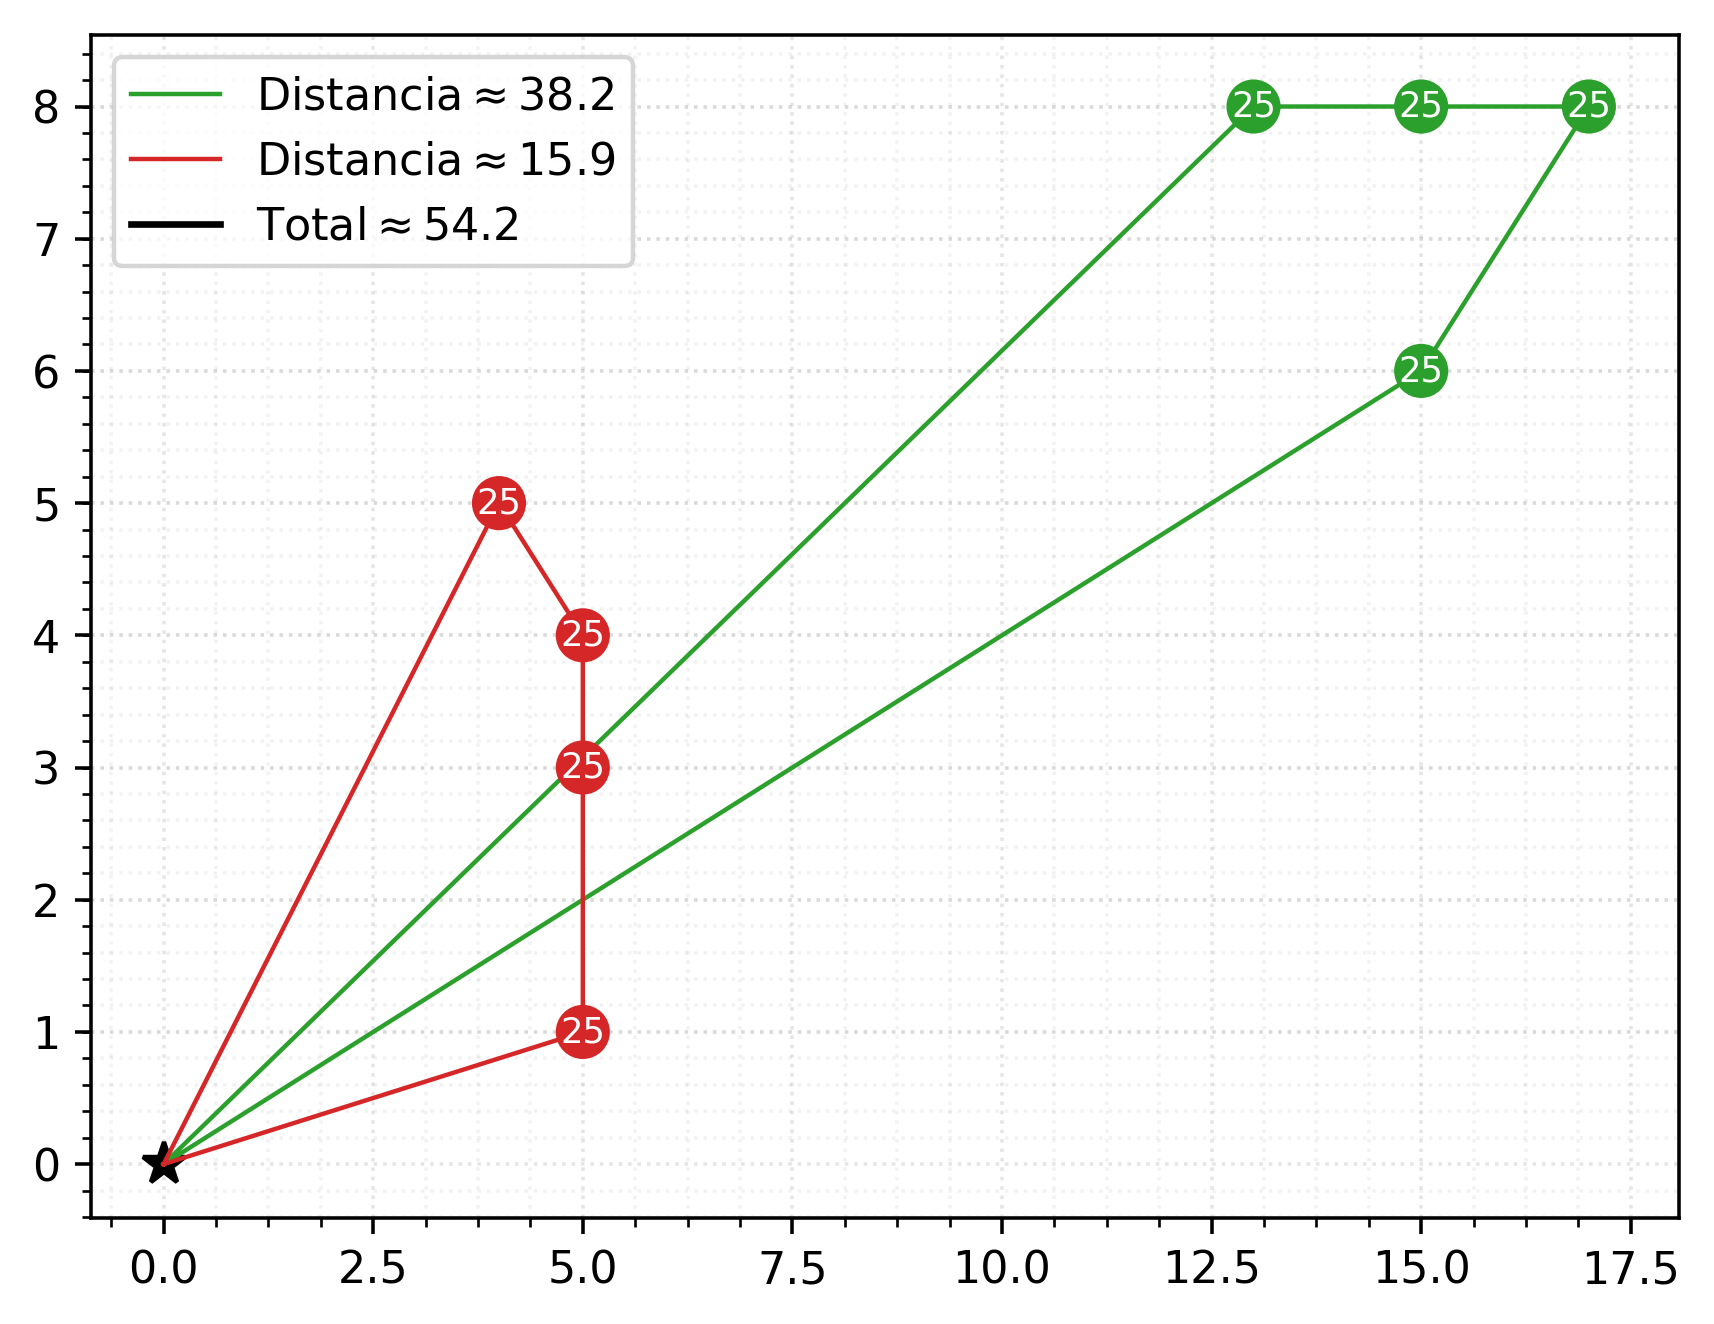
\includegraphics[width=1\textwidth]{sweep/km-custom-n9-sweep-close-angular-far-euclidean}
		\caption{\footnotesize K-Means + Nearest Neighbours. Capacidad 100.}
		\label{fig:km-custom-n9-sweep-close-angular-far-euclidean}
	\end{minipage}%
\end{figure}

En este caso se puede observar claramente lo mencionado. La solución con \textit{sweeping} encuentra primero el vértice $(5, 1)$ e inmediatamente después el $(15, 6)$, seguido del $(17, 8)$ y cierra el cluster con $(15, 8)$. Luego ya se disponen de 4 vértices cuya demanda suma $100$, la capacidad máxima de un camión. Esto forma un cluster de cuatro vértices donde uno de ellos está muy lejos de los otros tres pues estos cuatro son consecutivos angularmente pero \textbf{no} euclideanamente. Lo mismo sucede con los otros cuatro vértices sobrantes del grafo. En consecuencia, se consume mucha distancia yendo y viniendo de aquellos vértices lejanos del resto. En cambio, en la figura \ref{fig:km-custom-n9-sweep-close-angular-far-euclidean} se puede observar una distribución más natural de las rutas y, en consecuencia, un decremento en la distancia total recorrida por ellas. Esto se debe a que se utilizó la heurística de clusterización \textbf{K-Means} que resulta \textbf{más apropiada para la instancia del problema} pues – como será explicado más adelante – construye los clusters a partir de la distancia euclideana entre sus vértices y no sus distancias angulares al depósito.

